Habiendo expuesto cada uno de los pasos dentro de la metodología de la investigación en el capítulo anterior, 
en el presente capítulo se expondrán cada uno de los experimentos hechos de manera ordenada 
que se realizó. Primero se hablarán de los \textit{datasets} utilizados, los softwares y 
hardwares, el preprocesamiento de entradas. Finalmente, se abordarán los diferentes 
\textit{stages} del \textit{pipeline}, comenzando por el detector, luego el clasificador y 
terminando por el \textit{pipeline} completo.

\section{Aspectos generales}
\subsection{\textit{Datasets}}
Como ya había sido mencionado anteriormente, se utilizará un banco de imágenes de diferentes especies peruanas, las cuales fueron recogidas de  diferentes repositorios y competencias de la página \href{https://www.kaggle.com/}{\textit{Kaggle}}. Estos \textit{datasets}  contienen las imágenes de peces y sus \textit{labels}, los cuales representan las especies del pez que se encuentra dentro de la imagen. Se obtuvieron 3 diferentes \textit{datasets}, de entre los cuales se extrajeron únicamente las especies que también se encuentran en el mar peruano y de entre ellos, el primero se utilizará para la comprobación del \textit{pipeline} final, mientras que los otros dos se utilizaron para probar el clasificador. La lista de cada uno de los \textit{datasets} se encuentra a continuación:
\begin{itemize}
    \item \href{https://www.kaggle.com/c/the-nature-conservancy-fisheries-monitoring}{\textit{The Nature Conservancy Fisheries Monitoring}}: Concurso realizado en 2017 a través de la plataforma mencionado anteriormente. Contiene varias imágenes sobre las siguientes especies: atún blanco o ``bonito'', atún de ojo grande, atún de aleta amarilla y pez delfín o comúnmente llamado ``perico''.
    \item \href{https://www.kaggle.com/datasets/giannisgeorgiou/fish-species}{\textit{Fish Species}}: Contiene 2000 imágenes de cada una de las 20 especies del mediterráneo de entre las cuales se ha recolectado las imágenes de la lisa o ``Mugil cephalus'', el pez guitarra o ``Rhinobatos cemiculus'', la caballa o ``scomber japonicus'' y el pez espada o ``tetrapturus belone'' . 
    \item \href{https://www.kaggle.com/datasets/crowww/a-large-scale-fish-dataset}{\textit{A Large Scale Fish Dataset}}: Contiene 1000 imágenes de 9 especies diferentes encontradas en Turquía, de entre las cuales, una de ellas, la trucha marrón, también se encuentra en aguas peruanas. 
\end{itemize}

\subsection{Software y Hardware}
A lo largo de toda la experimentación, se utilizará un computador de escritorio con las siguientes características:

\begin{table}[h!]
\centering
\footnotesize
\begin{tabular}{|l|l|}
\hline
\textbf{Componente} & \textbf{Descripción} \\ \hline
Procesador & AMD Ryzen 7 3700X 8-Core 3.6 GHz. \\ \hline
Memoria RAM & Crucial Ballistix 16GB DDR4 - 3600MHZ \\ \hline
Tarjeta Gráfica & Nvidia RTX 2060 6GB \\ \hline
\end{tabular}
\end{table}

Por otra parte, se utilizó Python, junto con Keras, Sklearn y Tensorflow 
para el desarrollo del \textit{pipeline} en general y el pre y post 
procesamiento de los datos. Para el procesamiento de las imágenes (con Yolo) 
se utilizó OpenCV compilado con cudnn para la habilitación del uso de tarjeta gráfica. 

\subsection{Preprocesamiento de \textit{Bounding Boxes}}

Se llevó a cabo la creación manual de los \textit{bounding boxes} para todas las 
imágenes del \textit{dataset} ``\textit{The Nature Conservancy}'', utilizando el 
software de código abierto \textit{YoloLabel}, el cual proporciona una interfaz 
sencilla. Se contó con ayuda de un experto para crear los \textit{bounding boxes} 
y etiquetar cada imagen.
\\\\
Es importante mencionar que, aunque las imágenes en general eran borrosas, las del 
conjunto de entrenamiento resultaron ser menos complejas que las del conjunto de 
prueba. De hecho, estas últimas fueron difíciles de clasificar incluso para el 
experto. Una vez creados los \textit{bounding boxes}, se procedió a recortar las 
imágenes. Como resultado de este proceso, se obtuvieron diferentes cantidades de 
imágenes por clase, como se muestra en la tabla \ref{table:ImagenesNumero}:
\\
\begin{table}[h!]
\footnotesize
\centering
\begin{tabular}{|c|r|r|}
\hline
Especie                                                            & \multicolumn{1}{c|}{\begin{tabular}[c]{@{}c@{}}Número de\\ imágenes de\\ entrenamiento\end{tabular}} & \multicolumn{1}{c|}{\begin{tabular}[c]{@{}c@{}}Número de\\ imágenes de\\ prueba\end{tabular}} \\ \hline
\textit{\begin{tabular}[c]{@{}c@{}}Albacore \\ Tuna\end{tabular}}  & 2341                                                                                                 & 383                                                                                           \\ \hline
\textit{\begin{tabular}[c]{@{}c@{}}Bigeye \\ Tuna\end{tabular}}    & 288                                                                                                  & 391                                                                                           \\ \hline
\textit{Dolphinfish}                                               & 127                                                                                                  & 20                                                                                            \\ \hline
\textit{\begin{tabular}[c]{@{}c@{}}Moonfish \\ (LAG)\end{tabular}} & 98                                                                                                   & 59                                                                                            \\ \hline
\textit{Shark}                                                     & 300                                                                                                  & 131                                                                                           \\ \hline
\textit{\begin{tabular}[c]{@{}c@{}}Yellowfin \\ Tuna\end{tabular}} & 195                                                                                                  & 21                                                                                            \\ \hline
\textit{Other}                                                     & 778                                                                                                  & 164                                                                                           \\ \hline
\textit{\textbf{Total}}                                            & \textbf{4127}                                                                                        & \textbf{1169}                                                                                 \\ \hline
\end{tabular}
\caption{Número de imágenes por \textit{dataset}}
\label{table:ImagenesNumero}
\end{table}

Una observación crucial que debe ser mencionada es la presencia de heterogeneidad en 
ambos \textit{datasets}, lo cual se asemeja a la realidad, ya que algunos de los peces 
son más difíciles de capturar que otros. Por lo tanto, este caso de estudio también involucra otros desafíos, como clases desequilibradas y un número bajo de imágenes, lo que puede provocar \textit{overfitting} en muchos casos, ya que debido a la disparidad de clases y la complejidad de los modelos, existe la posibilidad que se categorice las clases con más instancias \cite{Overfitting}.

\section{Evaluación de Detectores }
En esta primera experimentación se realizarán pruebas con 3 diferentes modelos: Yolov5 
preentrenado con el \textit{dataset} ``Objects 365'', UniDet y Yolov5 entrenado con 
nuestro \textit{dataset}. Para ello, se obtuvo un conjunto aleatorio del 80\% y 20\% de 
las imágenes recortadas entre el conjunto de entrenamiento y prueba, mientras que para el 
entrenamiento del Yolov5, se utilizaron todos los datos de entrenamiento y prueba.

\subsection{Extracción de imágenes por el detector} 
Una vez obtenidos el 80\% y 20\% de las imágenes del \textit{dataset} 
``\textit{The Nature Conservancy}'' en donde se unificaron los \textit{datasets} de entrenamiento 
y prueba (acción que se justificará en la sección 5.4.1 y que está evidenciada en el anexo 
\ref{appendix}). se utilizaron tres diferentes detectores para el recorte de las imágenes. 
Para cada uno de ellos, se clasificaron los recortes por la etiqueta de la imagen de la cual 
fueron obtenidas y las que eran de prueba fueron nuevamente etiquetados por el experto. Por 
otra parte, todas las imágenes recortadas que no contenían un pez dentro, no estaban enfocadas 
o no contenían perfectamente al pez y fueron etiquetadas como errores. Para esta experimentación 
se utilizaron dos yolov5 (uno preentrenado con Objects365 y uno entrenado con el \textit{dataset}) 
y un UniDet, entrenado con COCO, Objects 365 y OpenImages. Los datos obtenidos fueron 
recopilados en la tabla \ref{table:peces}. Cabe resaltar que el yolov5 entrenado fue utilizado 
como detector general (ignorando las clases que predecía).
\\
\begin{table}[h!]
\footnotesize
\centering
\begin{tabular}{|c|r|r|r|}
\hline
\multicolumn{1}{|r|}{}                                                                                     & \multicolumn{1}{c|}{Peces detectados} & \multicolumn{1}{c|}{\begin{tabular}[c]{@{}c@{}}Otros objetos\\ (errores)\end{tabular}} & \multicolumn{1}{c|}{\textbf{Total}} \\ \hline
Real                                                                                                       & 1061                                  & -                                                                                     & \textbf{1061}                       \\ \hline
\begin{tabular}[c]{@{}c@{}}Predicted Yolov5\\ pretrained(40\%\\ threshold)\end{tabular}                    & 150                                   & 335                                                                                   & \textbf{485}                        \\ \hline
\begin{tabular}[c]{@{}c@{}}Predicted UniDet\\ pretrained (no \\ threshold)\end{tabular}                    & 426                                   & 124                                                                                   & \textbf{550}                        \\ \hline
\begin{tabular}[c]{@{}c@{}}Predicted Yolov5\\ trained (freezed \\ backbone 95\% \\ threshold)\end{tabular} & 843                                   & 399                                                                                   & \textbf{1233}                       \\ \hline
\end{tabular}
\caption{Número de peces vs errores detectados por cada modelo}
\label{table:peces}
\end{table}

Como se esperaba, utilizar un modelo preentrenado no especializado en detectar una clase específica, genera una menor precisión en comparación de uno que sí está entrenado, y más aún, si ese \textit{dataset} es el que está usando para clasificar. Se utilizaron dos métricas para el análisis de estos datos: el porcentaje de peces detectados con respecto del \textit{dataset} original y el porcentaje de error general obtenido por cada detección. Estos resultados se pueden ver en la tabla \ref{table:pecesPorcentaje}.
\\

\begin{table}[h!]
\footnotesize
\centering
\begin{tabular}{|c|r|r|}
\hline
\multicolumn{1}{|r|}{}                                                                                     & \multicolumn{1}{c|}{\begin{tabular}[c]{@{}c@{}}Porcentaje de\\ peces detectados\end{tabular}} & \multicolumn{1}{c|}{\begin{tabular}[c]{@{}c@{}}Porcentaje de errores\\ detectados del total\end{tabular}} \\ \hline
\begin{tabular}[c]{@{}c@{}}Predicted Yolov5\\ pretrained(40\%\\ threshold)\end{tabular}                    & 14.13\%                                                                                       & 69.07\%                                                                                                   \\ \hline
\begin{tabular}[c]{@{}c@{}}Predicted UniDet\\ pretrained (no \\ threshold)\end{tabular}                    & 40.15\%                                                                                       & \textbf{22.54\%}                                                                                                   \\ \hline
\begin{tabular}[c]{@{}c@{}}Predicted Yolov5\\ trained (freezed \\ backbone 95\% \\ threshold)\end{tabular} & \textbf{79.45\%}                                                                                       & 32.36\%                                                                                                   \\ \hline
\end{tabular}
\caption{Porcentaje de detecciones correctas vs errores generados }
\label{table:pecesPorcentaje}
\end{table}

Se puede ver una baja precisión por parte del Yolov5 preentrenado, lo cual es comprensible considerando que no ha sido preentrenado especialmente para detectar peces, sino con un \textit{dataset} genérico y es un modelo bastante ligero. UniDet, en cambio, es un modelo mucho más complejo, y tiene 3 detectores internamente (uno para cada dataset), los cuales en conjunto predicen la clase final del objeto y es por lo cual generan un mejor resultado que el anterior pero a un costo mucho mayor. Finalmente el Yolov5 entrenado específicamente con el \textit{dataset} obtenido muestra una especialización en la detección de estos individuos que finalmente logra un 79.45\% de precisión. Aún así se necesita considerar el hecho que el entrenamiento de este modelo tomo alrededor de 80 minutos, siendo este aproximadamente 13 veces más el tiempo que le toma entrenar a un modelo como lo es EfficientnetB0 con un bajo número de imágenes(4300 imágenes, a comparación de 5300 para el CNN).
\\\\

Además, al considerar el porcentaje de errores generados, se observa que UniDet produce una menor cantidad de detecciones incorrectas en comparación con \textit{pretrained} YOLOv5 y \textit{trained} YOLOv5, lo que demuestra que es un modelo más robusto. Sin embargo, debido a la falta de especialización durante su entrenamiento, UniDet ofrece resultados más pobres en las detecciones. En este sentido, se cree que si tuviéramos los pesos de un modelo específicamente entrenado para la detección de peces, se mejoraría el resultado y se evitaría la necesidad de entrenar uno desde cero o utilizar uno que haya sido entrenado de manera genérica. Esto aumentaría la precisión general del sistema y tendría un impacto positivo en el flujo de trabajo.
\\\\

\section{Evaluación de Desempeño de Diferentes Clasificadores}
En la presente sección se realizarán dos experimentos para poder seleccionar una arquitectura que será utilizada para actuar como nuestro clasificador dentro del \textit{pipeline} final. Para ello, se compararán algunas arquitecturas del estado del arte utilizando los 3 \textit{datasets}, analizando tanto las pérdidas y precisión en \textit{training}, \textit{validation} y \textit{testing} para cada uno, así como la velocidad por batch (8 imágenes) y el número de épocas necesarias para entrenar dichas arquitecturas. 
\subsection{Arquitectura general}
Como fue mencionado, para la creación de cada una de las arquitecturas se utilizarán modelos ya preentrenados del estado del arte, a los cuales se les aplicará TL para su entrenamiento con nuestro \textit{dataset}. Este proceso consistirá en congelar todas las capas convolucionales, para luego ser pasado por una capa de \textit{GlobalAveragePooling2D}, luego por una \textit{Flatten}, la cual pasa de un formato bidimensional a uno unidimensional y luego por las siguientes tres capas: 
\begin{itemize}
    \item \textit{BatchNormalization}
    \item \textit{Dropout} de 50\%
    \item Capa densa a X \textit{outputs} con una función de activación RELU o softmax, dependiendo si es una capa oculta o la de salida.  
    \item 8 imágenes por batch 
\end{itemize}

Estas tres capas son ejecutadas para cada uno de los siguientes tamaños: $[1024,256,64,LABELS\_SIZE]$, donde LABELS\_SIZE representará el número de clases de salida que generará el clasificador.  

\subsection{Experimentación \#1}

Para el primer análisis, se utilizaron las consideraciones anteriores para comparar las diferentes arquitecturas del estado del arte mencionadas en el anterior capítulo. Para esta comparación, se utilizaron las imágenes obtenidas de los \textit{datasets} \textit{Fish Species} y \textit{A Large Scale Fish Dataset} combinados y se compararon los resultados de las métricas obtenidas. 
La primera de las métricas a comparar serán las gráficas de pérdida. En la figura \ref{fig:losses1} se ilustra una comparativa de la disminución de la pérdida con respecto al tiempo (épocas).

\begin{figure}[h!]
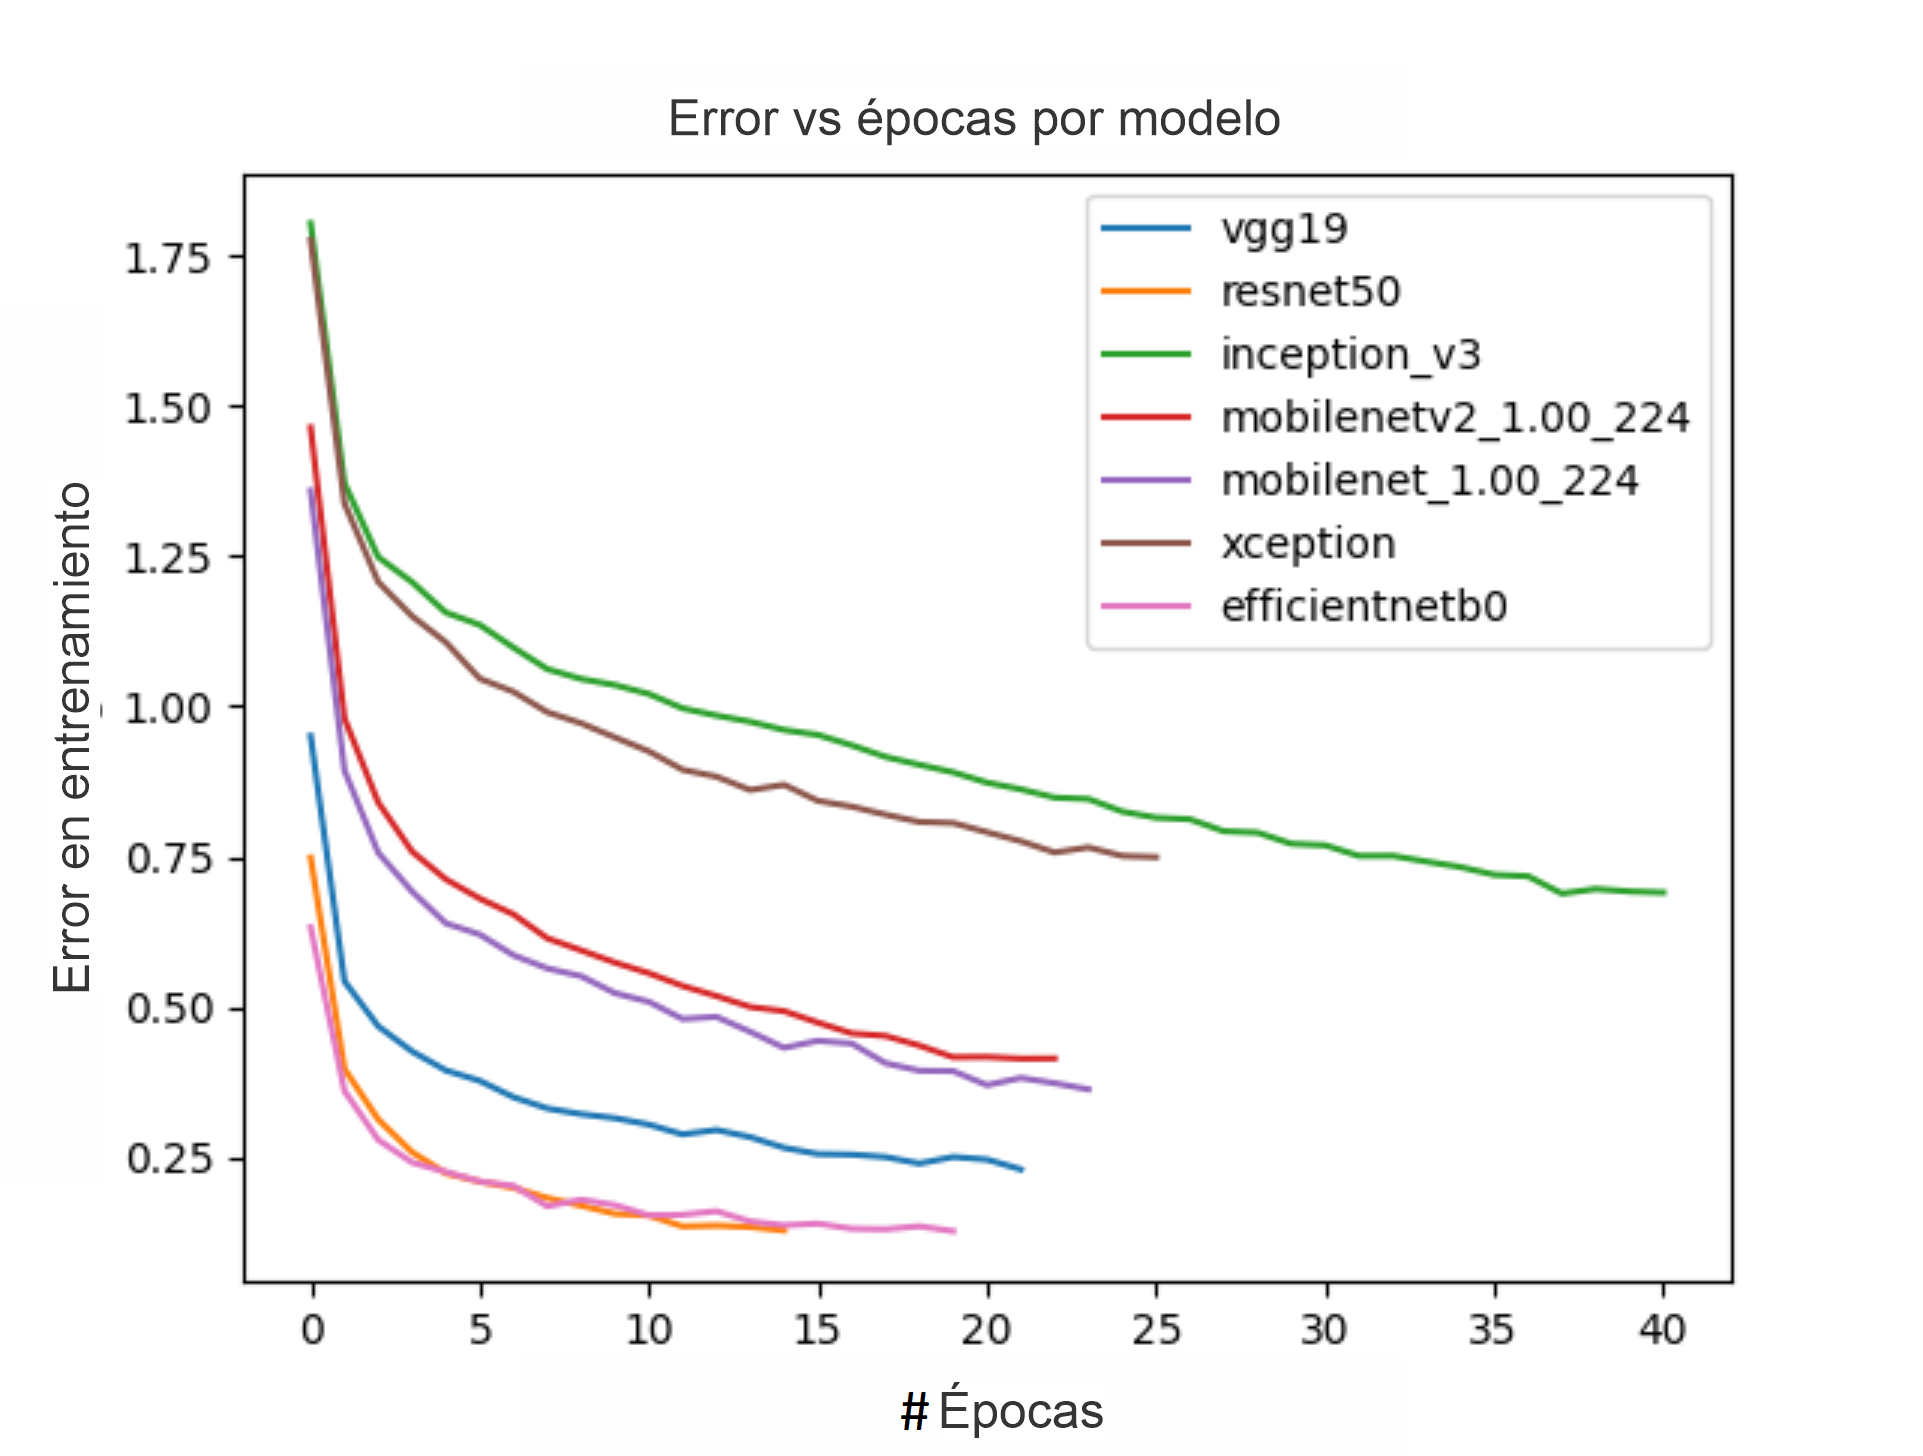
\includegraphics[width=1\textwidth]{images/loss1.png}
\centering
\caption{Gráfica comparativa de la pérdida entre todos los modelos a estudiar}
\label{fig:losses1}
\end{figure}


En esta gráfica se puede ver que los modelos que consiguen mejores descensos en esta 
métrica son tanto Resnet50, Vgg19 y EfficientnetB0, lo cual era bastante esperado conforme 
a la teoría, salvo por el Vgg19. Otro detalle interesante que salió a relucir de esta 
experimentación fue que InceptionV3 y Xception tuvieron una pérdida bastante elevada, 
contrario a lo que se esperaba en un inicio, lo cual podría ser motivo de análisis en un 
futuro para saber cuales fueron los motivos por los cuales no consiguieron aprender del 
\textit{dataset}. Por último, se puede ver como las dos MobileNet están en el medio de 
todas las demás redes analizadas, lo cual, es un dato a resaltar considerando lo ligero que 
son. \\\\

También se obtuvieron las siguientes métricas que fueron recopiladas en la tabla \ref{table:data1}.

\begin{table}[h!]
\footnotesize
\begin{tabular}{|c|c|c|c|c|c|c|}
\hline
\textbf{} & \textbf{\begin{tabular}[c]{@{}c@{}}Precisión\\en\\training\end{tabular}} & \textbf{\begin{tabular}[c]{@{}c@{}}Precisión \\ en \\ validation\end{tabular}} & \textbf{\begin{tabular}[c]{@{}c@{}}Precisión \\ en \\testing\end{tabular}} & \textbf{\begin{tabular}[c]{@{}c@{}}Perdida \\ final en \\ training\end{tabular}} & \textbf{\begin{tabular}[c]{@{}c@{}}Velocidad \\ por batch\\ (8 \\imágenes) \\ en ms\end{tabular}} & \textbf{\begin{tabular}[c]{@{}c@{}}Número \\ de\\ épocas\end{tabular}} \\ \hline
\textbf{Vgg19} & 0.9193 & 0.9928 & 0.9926 & 0.2299 & 71 & 21 \\ \hline
\textbf{Resnet50} & \textbf{0.9596} & \textbf{0.9993} & 0.9950 & 0.1282 & 52 & 14 \\ \hline
\textbf{\begin{tabular}[c]{@{}c@{}}Inception\\V3\end{tabular}} & 0.7362 & 0.6620 & 0.6681 & 0.6901 & 42 & 40 \\ \hline
\textbf{\begin{tabular}[c]{@{}c@{}}MobileNet\\V2\end{tabular}} & 0.8521 & 0.9052 & 0.9104 & 0.4143 & 28 & 31 \\ \hline
\textbf{\begin{tabular}[c]{@{}c@{}}MobileNet\\V1\end{tabular}} & 0.8694 & 0.9288 & 0.9519 & 0.3628 & \textbf{23} & 23 \\ \hline
\textbf{Xception} & 0.7244 & 0.7085 & 0.7178 & 0.7490 & 48 & 25 \\ \hline
\textbf{\begin{tabular}[c]{@{}c@{}}EfficientNet\\B0\end{tabular}} & 0.9577 & \textbf{0.9993} & \textbf{1.0000} & \textbf{0.1270} & 41 & \textbf{19} \\ \hline
\end{tabular}
\caption{Datos recopilados de la prueba de diferentes modelos del estado del arte}
\label{table:data1}
\end{table}


Esta tabla también proporciona datos interesantes sobre la experimentación. En primer lugar, 
Vgg19 tuvo la mayor pérdida entre todos los modelos, pero logró una precisión bastante 
aceptable en términos de entrenamiento, mientras que su precisión en validación y prueba 
fue casi perfecta. En segundo lugar, siguiendo con el análisis anterior, se observa que 
InceptionV3 y Xception obtuvieron resultados acordes a su pérdida en términos de precisión 
general. \\\\
Otro punto a resaltar es el hecho que ambos MobileNet obtienen un resultado bastante similar 
en términos de precisión en general, pero MobileNetV2 obtiene una pequeña diferencia, la cual 
la hace mejor que su versión anterior, pero a un costo en términos de velocidad, lo cual 
también se esperaba conforme a la teoría. Por último, cabe señalar que los tres modelos que 
obtuvieron la mejor precisión en pruebas fueron EfficientnetB0, Resnet50 y Vgg19 respectivamente.\\\\
A manera de conclusión, se pudo ver que con un \textit{dataset} relativamente sencillo, se puede obtener resultados bastante favorables, que logran casi a su totalidad automatizar este tipo de problemas con modelos ya pre-entrenados que son facilmente modificables para su uso.

\subsection{Experimentación \#2}

Para este segundo análisis, se  utilizaron las imágenes obtenidas del \textit{datasets} 
\textit{The Nature Conservancy Fisheries Monitoring}. Dentro de estas imágenes se podrían 
encontrar muchos peces de la misma especie por imagen. En ese sentido la labor del 
clasificador será identificar si esta imagen contiene ejemplares de un determinado 
pez en ella. Para este experimento, únicamente se tomaron los \textit{datasets} de 
entrenamiento y validación, ya que el de testeo no contenía etiquetas, pero será 
utilizado en futuras experimentaciones.  De la misma manera que en la anterior 
experimentación, primero se procederá a analizar las gráficas de error, tal como se 
ven en la imagen \ref{fig:losses2}.
\begin{figure}[h!]
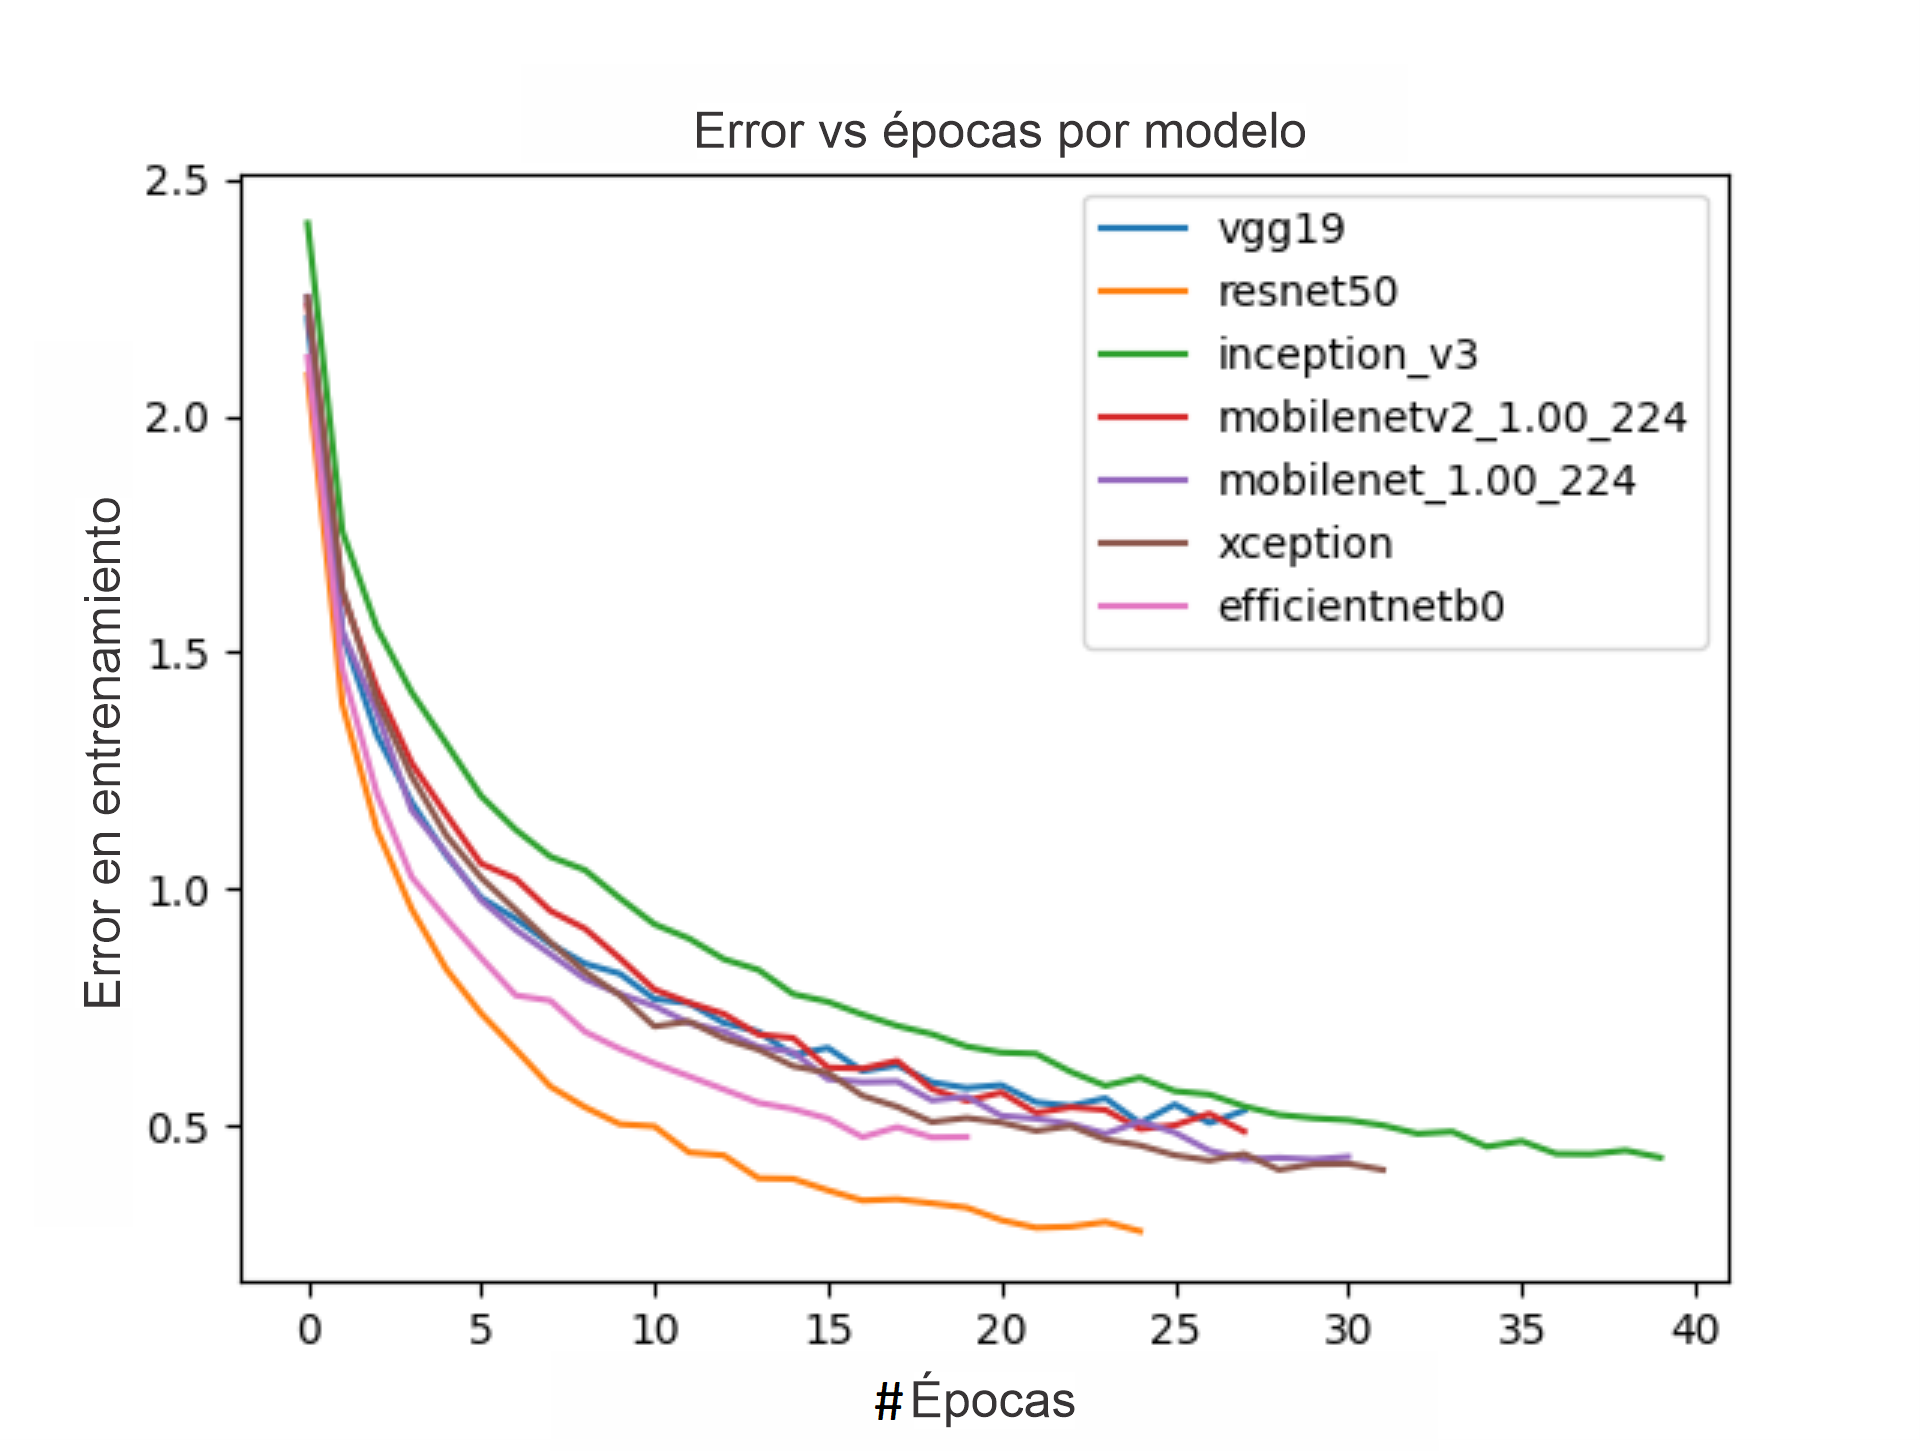
\includegraphics[width=1\textwidth]{images/loss2.png}
\centering
\caption{Gráfica comparativa de la perdida entre todos los modelos a estudiar}
\label{fig:losses2}
\end{figure}
Se puede ver que en esta experimentación se tuvieron rangos de error más elevados que el anterior, esto debido a la complejidad de la tarea. También se puede ver un descenso del error bastante más parejo entre todos los modelos experimentados. Nuevamente aparecen Resnet50 y Efficientnet con los menores resultados y también un menor número de épocas necesitadas para este entrenamiento.\\\\
Ahora pasaremos a analizar las métricas obtenidas para estos modelos, los cuales están plasmados en la tabla \ref{table:data2}.
\newpage
\begin{table}[h!]
\footnotesize
\begin{tabular}{|c|c|c|c|c|c|}
\hline
\textbf{} & \textbf{\begin{tabular}[c]{@{}c@{}}Precisión\\  en training\end{tabular}} & \textbf{\begin{tabular}[c]{@{}c@{}}Precisión \\ en \\ validation\end{tabular}} & \textbf{\begin{tabular}[c]{@{}c@{}}Perdida \\ final en \\ training\end{tabular}} & \textbf{\begin{tabular}[c]{@{}c@{}}Velocidad \\ por batch\\ ( 8 \\imágenes) \\ en ms\end{tabular}} & \textbf{\begin{tabular}[c]{@{}c@{}}Número \\ de\\ épocas\end{tabular}} \\ \hline
\textbf{Vgg19} & 0.8173 & 0.9061 & 0.5317 & 68 & 29 \\ \hline
\textbf{Resnet50} & \textbf{0.9139} & \textbf{0.9219} & \textbf{0.2769} & 50 & 24 \\ \hline
\textbf{\begin{tabular}[c]{@{}c@{}}Inception \\ V3\end{tabular}} & 0.8510 & 0.8637 & 0.4324 & 42 & 39 \\ \hline
\textbf{\begin{tabular}[c]{@{}c@{}}MobileNet\\V2\end{tabular}} & 0.8348 & 0.8516 & 0.4875 & 28 & 27 \\ \hline
\textbf{\begin{tabular}[c]{@{}c@{}}MobileNet\\V1\end{tabular}} & 0.8543 & 0.8743 & 0.4340 & \textbf{24} & 30 \\ \hline
\textbf{Xception} & 0.8676 & 0.8267 & 0.4065 & 48 & 31 \\ \hline
\textbf{\begin{tabular}[c]{@{}c@{}}EfficientNet\\B0\end{tabular}} & 0.8467 & \textbf{0.9101} & 0.4759 & 41 & \textbf{19} \\ \hline
\end{tabular}
\caption{Datos recopilados de la prueba de diferentes modelos del estado del arte}
\label{table:data2}
\end{table}

En comparación con la gráfica anterior, se observa un deterioro en todas las métricas obtenidas. Resnet y Efficientnet mostraron una alta precisión en entrenamiento y validación, superando a Vgg19, el cual no obtuvo una buena precisión en entrenamiento y presentó una alta pérdida final, lo cual sugiere que sufrió de \textit{overfitting}. Si consideramos además la relación entre precisión y eficiencia, ambas MobileNet resultan bastante robustas, ya que generan una precisión relativamente alta, manteniendo una velocidad por \textit{batch} razonable. Exceptuando ambas MobileNets, InceptionV3 y EfficiententB0 fueron las que obtuvieron una velocidad por \textit{batch} menor que las demás. Por último cabe resaltar que Resnet50 y Efficientnet fueron las redes que necesitaron un menor número de épocas para detenerse. 
\\\\
Considerando los resultados obtenidos, proponemos el uso de EfficientnetB0 para la creación del \textit{pipeline}, debido a su alta precisión tanto en las pruebas como en el entrenamiento, así como en la validación y prueba. Además, es significativamente más ligero, presenta una curva de aprendizaje más estable a lo largo de las épocas, un menor número de épocas necesitadas para entrenarse y una velocidad superior a todas las demás.

\section{Experimentación del clasificador}

En esta sección se llevaron a cabo 5 experimentos con el objetivo de validar y 
obtener un modelo entrenado basado en la arquitectura seleccionada en la sección anterior, 
con el fin de maximizar la precisión al entrenarlo con las imágenes recortadas. Dos de los 
experimentos se realizaron debido a una distribución inadecuada de los datos entre el 
\textit{dataset} de entrenamiento y el de pruebas. Estos dos experimentos se separaron y se 
mencionan en la sección de anexos para evitar interferencias con la continuidad de los demás 
experimentos.
\subsection{Experimentación \#1 (training/validation)}

En el primer experimento se emplearon únicamente las imágenes recortadas del \textit{dataset} 
de entrenamiento para comprobar la capacidad de aprendizaje del modelo. De estas imágenes, 
se seleccionó una parte para ser utilizada como conjunto de validación. En esta prueba, 
se llevaron a cabo 10 iteraciones utilizando el algoritmo de K-Fold para la muestra y se 
obtuvieron los resultados que se presentan en la tabla \ref{table:KFolds1}
\\

\begin{table}[h!]
\footnotesize
\centering
\begin{tabular}{|r|r|r|r|r|}
\hline
\textit{K} & \textit{training loss} & \textit{training accuracy} & \textit{validation loss} & \textit{validation accuracy} \\ \hline
1    & 0.0115      & 99.660\%    & 0.2697    & 94.43\%  \\ \hline
2    & 0.0011      & 100.00\%   & 0.2243    & 96.06\%  \\ \hline
3    & 0.0106      & 99.690\%    & 0.2106    & 95.13\%  \\ \hline
4    & 0.0186      & 99.510\%    & 0.2286    & 93.97\%  \\ \hline
5    & 0.0069      & 99.820\%    & 0.2265    & 95.36\%  \\ \hline
6    & 0.0060      & 99.820\%    & 0.1204    & 97.22\%  \\ \hline
7    & 0.0079      & 99.870\%    & 0.2417    & 91.88\%  \\ \hline
8    & 0.0147      & 99.640\%    & 0.2182    & 93.50\%  \\ \hline
9    & 0.0154      & 99.430\%    & 0.2767    & 93.27\%  \\ \hline
10   & 0.0327      & 98.920\%    & 0.2814    & 93.26\%  \\ \hline
\textbf{\textit{mean $\pm$ std}}     & \textbf{0.0125$\pm$0.0087}      & \textbf{99.636$\pm$0.304\%}    & \textbf{0.2298$\pm$0.0461}    & \textbf{94.41$\pm$1.567\%}  \\ \hline
\end{tabular}
\caption{Perdida y precisión de entrenamiento y validación}
\label{table:KFolds1}
\end{table}
Con estos resultados, podemos observar que al ejecutar el mismo modelo varias veces, se obtienen resultados similares, lo que demuestra que no hay \textit{overfitting} y que el modelo no ha sido influenciado por la aleatoriedad en la inicialización de los pesos. Además, al evaluar imágenes de manera individual, se logra aumentar la precisión del modelo en comparación con la clasificación de imágenes completas.
\\\\
A continuación, se procedió a experimentar con el \textit{dataset} de \textit{testing} para poder comprobar si el modelo generó buenos resultados al predecir las clases de las imágenes recortadas. Por el contrario, se comprobó que pertenecían a distribuciones de datos muy diferentes. En el \textit{dataset} de prueba se tenían imágenes en diferentes entornos, con menor visibilidad y mayor falta de características distintivas de las especies estudiadas, entre otros factores que dificultaban el aprendizaje. Para poder comprobarlo, se realizaron las experimentaciones A y B (detalladas en el anexo \ref{appendix}). Se obtuvo que el modelo predijo a las imágenes complejas como ``bonito'' (\textit{Albacore Tuna}), ya que en el \textit{dataset} de entrenamiento había una mayor cantidad de estas imágenes, por lo que era estadísticamente más probable acertar de ese modo. Además, estas imágenes eran las que presentaban más defectos dentro del conjunto. En ese sentido se cambio el enfoque de las experimentaciones siguientes.
\\\\
\subsection{Expermientación \#2 (extracción de datasets desde \textit{training}) }
Considerando lo anteriormente expuesto, se decidió dividir el conjunto de datos de entrenamiento en tres conjuntos diferentes: entrenamiento, validación y prueba, utilizando una proporción del 70\% para entrenamiento, 20\% para validación y 10\% para pruebas. El objetivo de esta nueva división fue comprobar si la suposición previa de que el problema era causado por el uso de conjuntos de datos con diferentes distribuciones era correcta. Los resultados obtenidos se muestran en la tabla \ref{table:Results4}.
\\
\begin{table}[h!]
\footnotesize
\centering
\begin{tabular}{|r|r|r|r|r|r|}
\hline
           & \multicolumn{1}{c|}{\textit{Loss}} & \multicolumn{1}{c|}{\textit{Balanced accuracy}} & \multicolumn{1}{c|}{\textit{F1-weighted}} & \multicolumn{1}{c|}{\textit{Precision}} & \multicolumn{1}{c|}{\textit{Recall}} \\ \hline
\textit{Train}      & 0.10                      & 96.57\%                        & 96.57\%                 & 96.76\%                         & 96.39\%                     \\ \hline
\textit{Validation} & 0.22                      & 95.64\%                        & 95.70\%                 & 95.75\%                         & 95.65\%                     \\ \hline
\textit{Testing}    & 0.23                      & 90.28\%                       & 95.29\%                & 95.39\%                       & 95.14\%                    \\ \hline
\end{tabular}
\caption{Estadísticos obtenidos del experimento \#2}
\label{table:Results4}
\end{table}

Se puede observar un comportamiento similar al experimento \#1, lo cual nos afirma entonces que realmente era un problema de malas distribuciones de datos en ambos \textit{datasets}. De la misma manera, se revisaron las matrices de confusión de los datos, los cuales se recopilaron en la tabla \ref{fig:Matrix2}

\begin{figure}[h!]
\centering
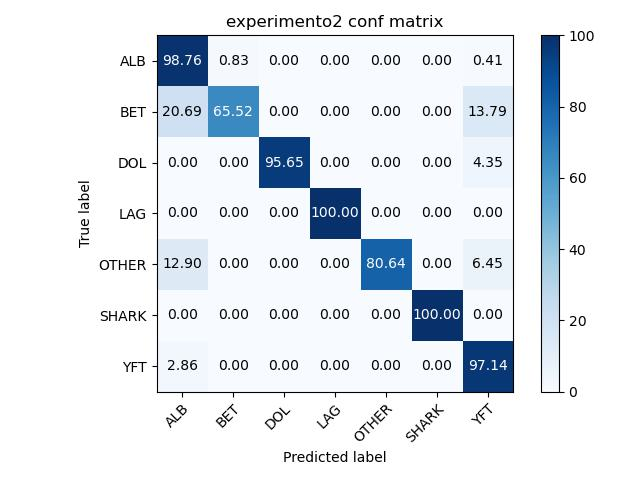
\includegraphics[width=0.8\textwidth]{images/experimento2_conf_matrix.jpg}
\caption{Matriz de confusión generada por el experimento \#2 en porcentajes}
\label{fig:Matrix2}
\end{figure}

Como se puede apreciar en la matriz de confusión, en general se obtuvo una buena precisión en la mayoría de las clases, excepto en la clase ``Bigeye Tuna'', lo cual es comprensible ya que se trata de una especie bastante similar al ``\textit{Albacore Tuna}'' y las imágenes no permiten apreciar las características diferenciales con claridad, como se pueden apreciar en las imágenes \ref{fig:combined2}.

\begin{figure}[h!]%
    \centering
    \subfloat[\centering Imagen de un ``bonito'' o ``\textit{Albacore Tuna}'' ]{{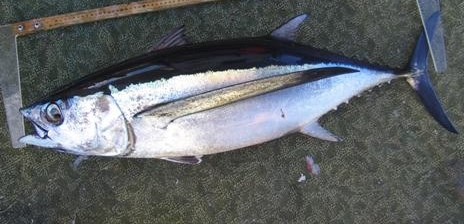
\includegraphics[width=5cm]{images/albacore.jpg} }}%
    \qquad
    \subfloat[\centering Imagen de un ``\textit{Bigeye Tuna}'']{{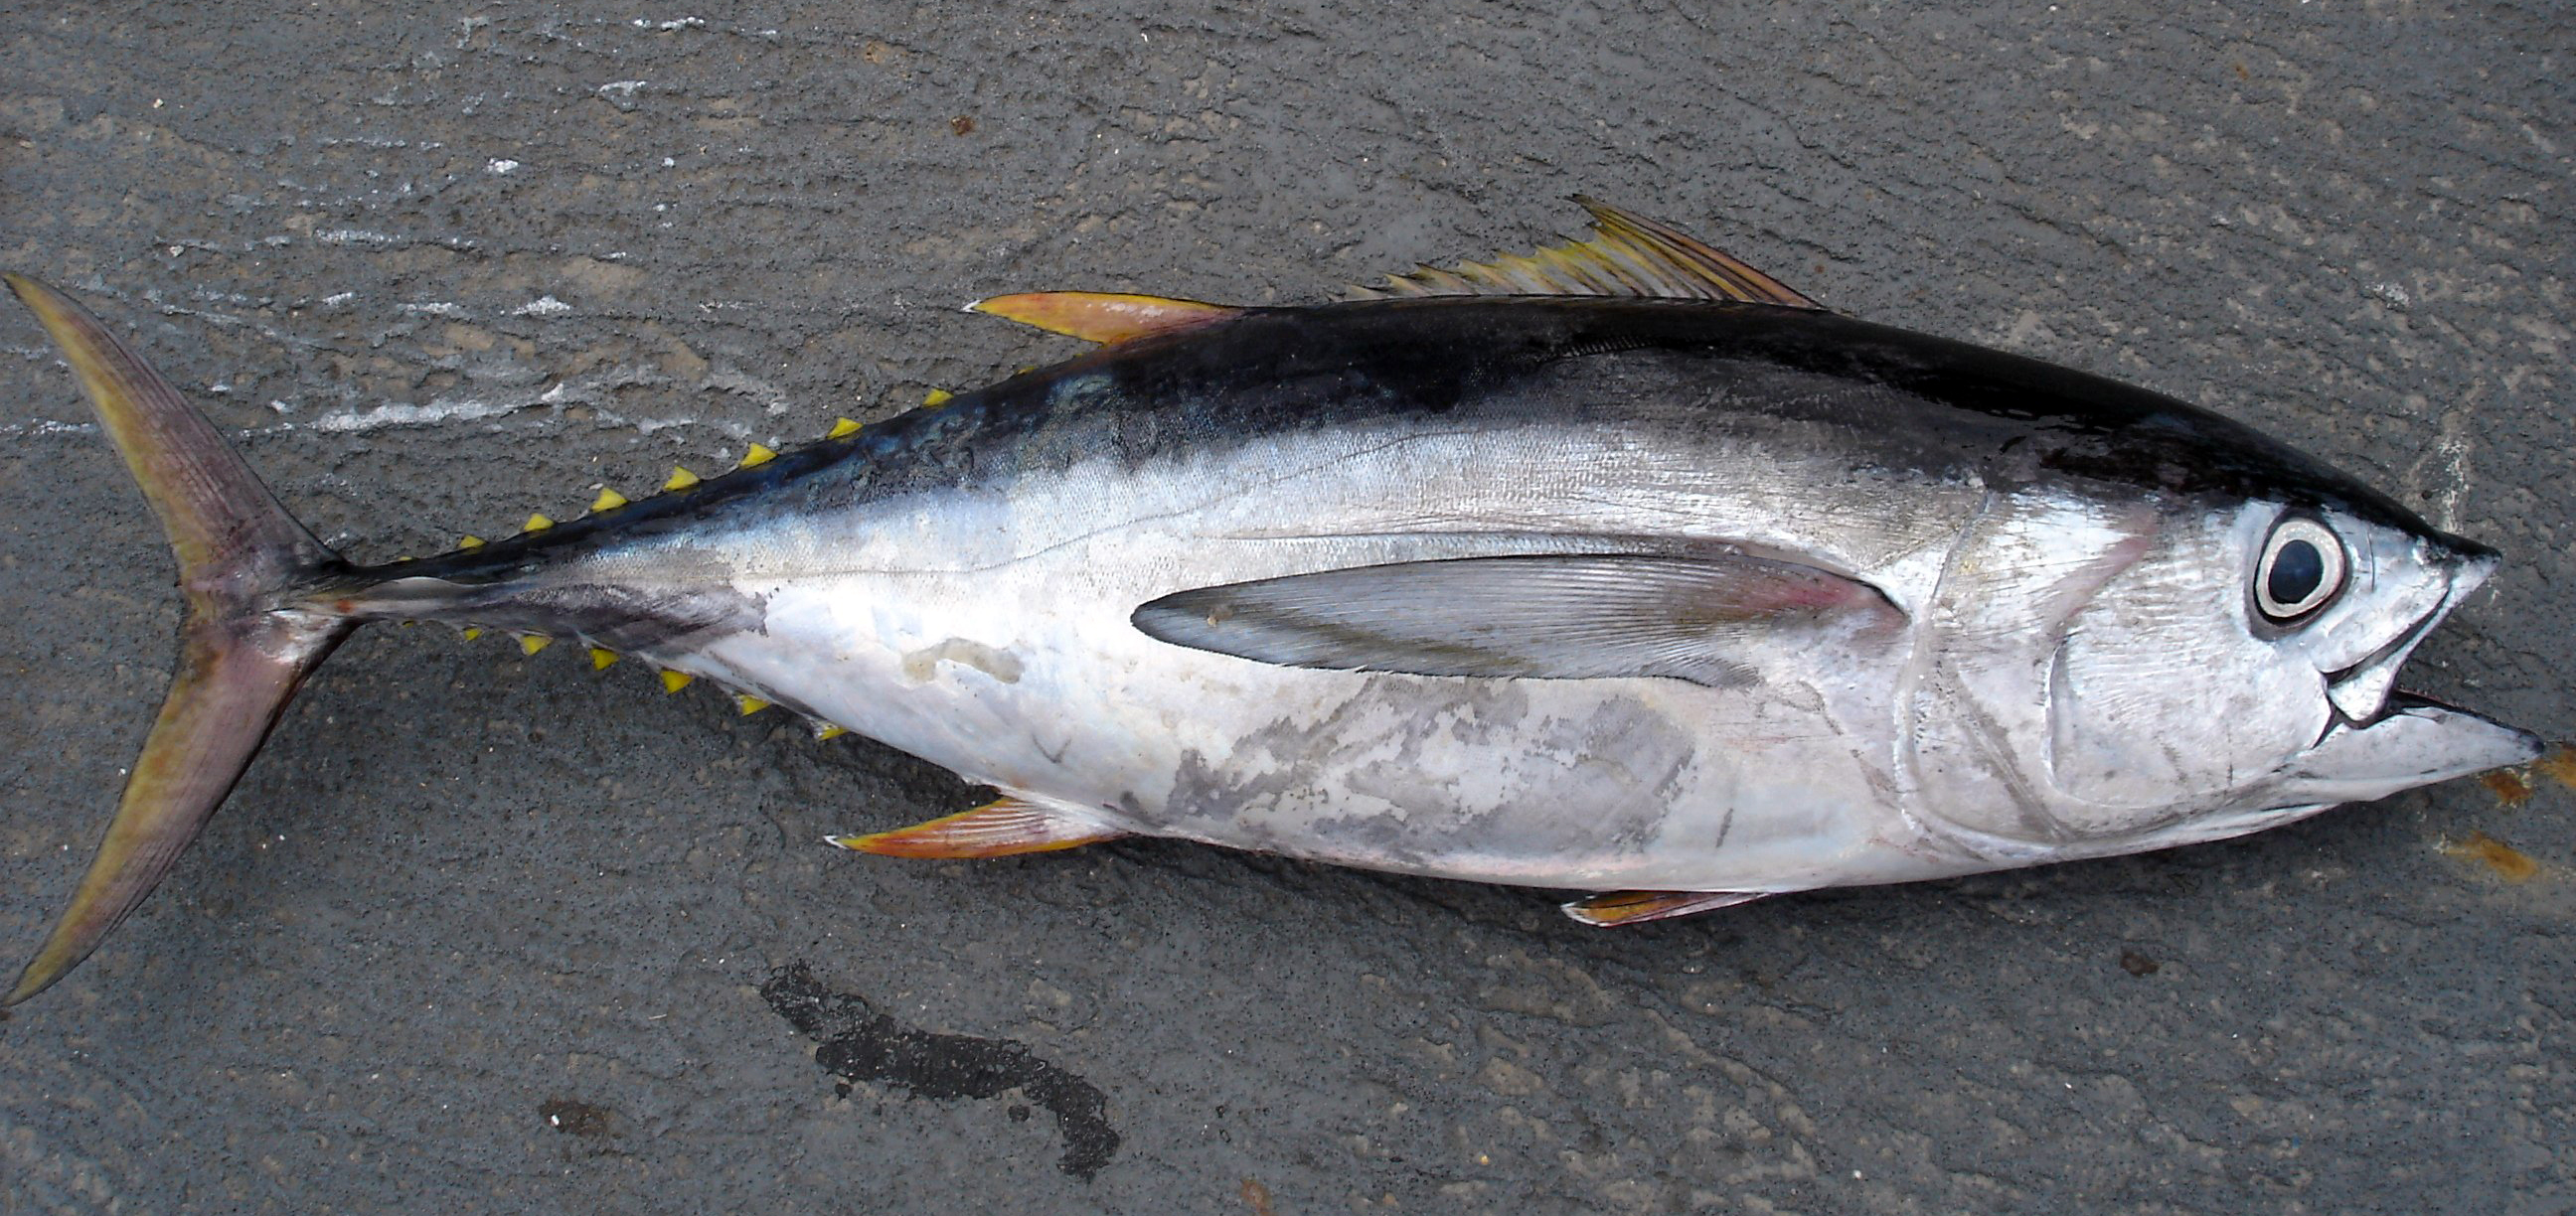
\includegraphics[width=5cm]{images/bigeye.jpg} }}%
    \caption{Comparación entren el ``\textit{Albacore Tuna}'' o bonito y el ``Bigeye Tuna''}%
    \label{fig:combined2}%
\end{figure}

 Además, se puede observar que no existe \textit{overfitting}, ya que las clases con menor cantidad de imágenes también consiguieron una alta precisión. También se revisaron las gráficas de pérdida y precisión tanto para el conjunto de entrenamiento como para el de validación, las cuales se muestran en las figuras \ref{fig:losses4} y \ref{fig:accuracy4}.
\\
\begin{figure}[h!]
\centering
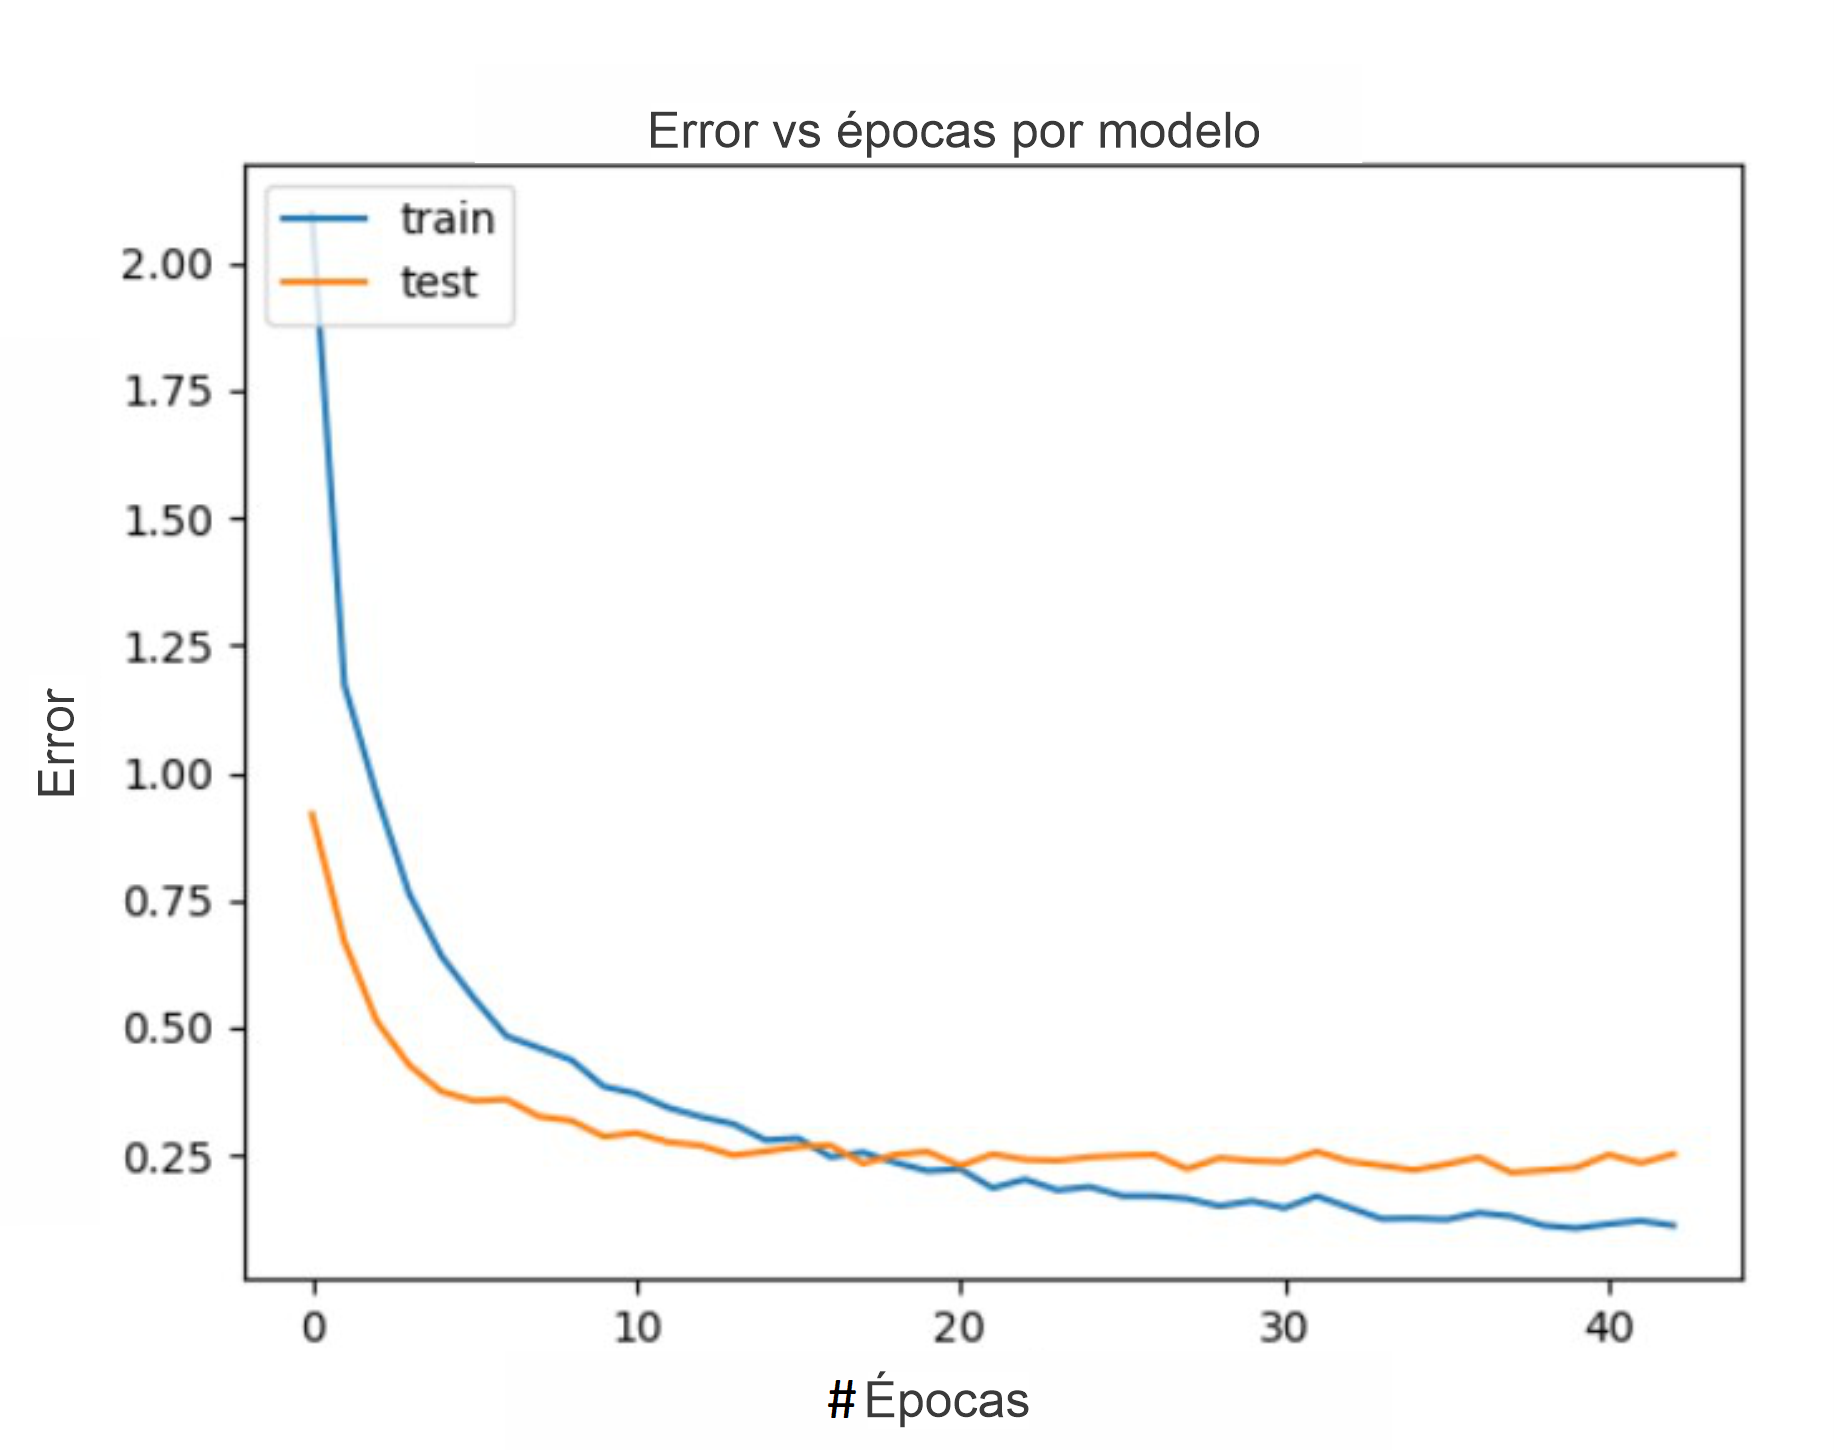
\includegraphics[width=0.8\textwidth]{images/loss4.png}
\caption{Gráfica comparativa de la perdida de entrenamiento y validacion}
\label{fig:losses4}
\end{figure}

\begin{figure}[h!]
\centering
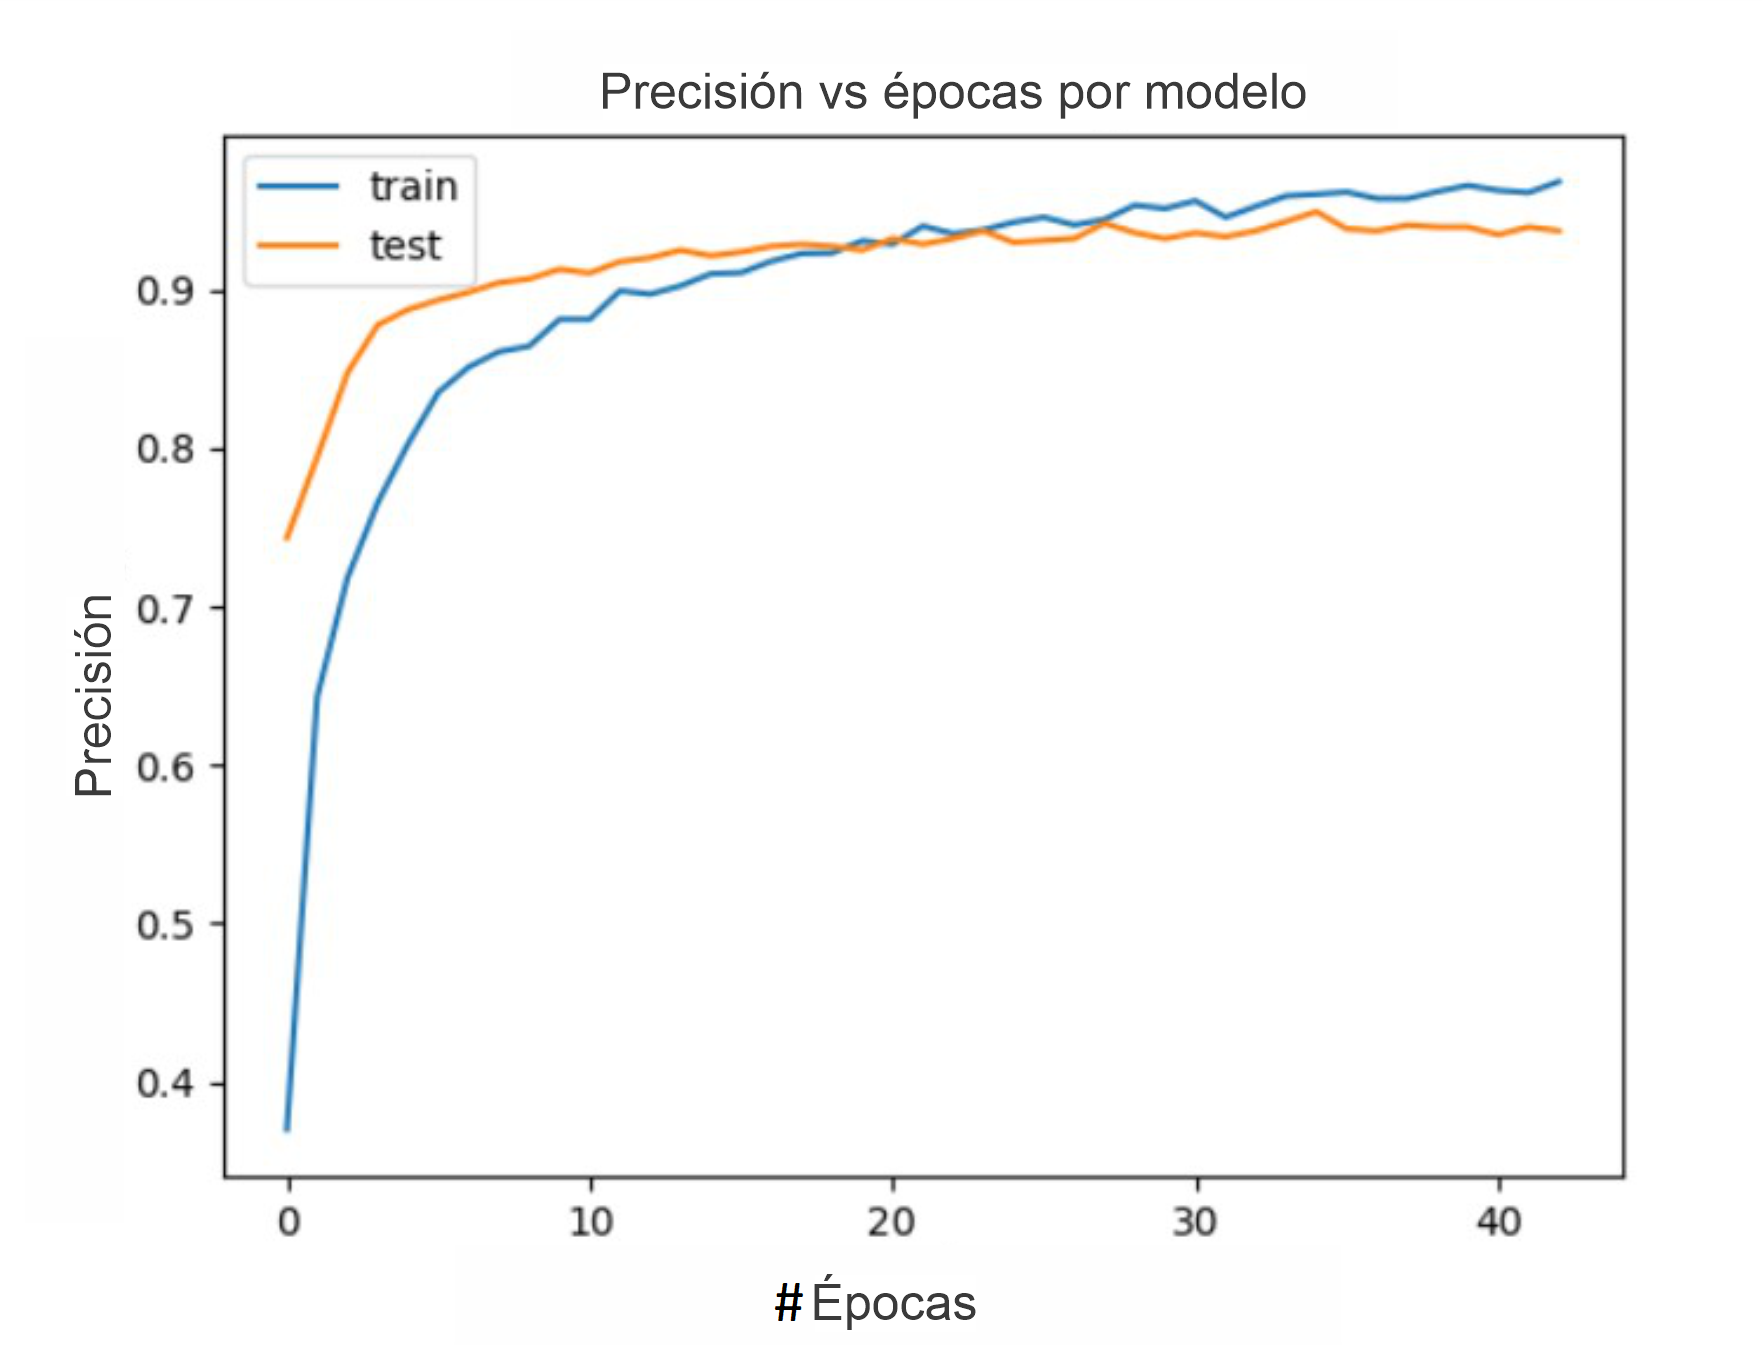
\includegraphics[width=0.8\textwidth]{images/accuracy4.png}
\caption{Gráfica comparativa de la precisión de entrenamiento y validacion}
\label{fig:accuracy4}
\end{figure}


Las gráficas muestran un aprendizaje constante, lo que refuerza la conclusión de que la red está aprendiendo correctamente, evitando aprender en exceso de ciertas clases e incluso obteniendo resultados positivos con las clases que tienen menor cantidad de imágenes. Además, es importante destacar que, en comparación con los experimentos previos del clasificador, estas nuevas redes podrían estar tardando más épocas en aprender de los datos debido a la complejidad de los mismos.

\subsection{Expermientación \#3 (extracción de datasets desde \textit{training}+\textit{testing})}
Con los resultados del anterior experimento se planteó unificar ambos \textit{datasets} y en base a esa nueva distribución de datos realizar la separación de los \textit{datasets }de \textit{training}, \textit{validation} y \textit{testing}. Dicha separación se realizó con los mismos porcentajes del anterior experimento. Al ejecutar la prueba, se obtuvieron los resultados de la tabla \ref{table:Results5}


\begin{table}[h!]
\centering
\begin{tabular}{|r|r|r|r|r|r|}
\hline
\textit{}           & \multicolumn{1}{c|}{\textit{Loss}} & {\textit{\begin{tabular}[c]{@{}c@{}}Balanced\\ Accuracy\end{tabular}}} & \multicolumn{1}{c|}{\textit{F1-weighted}} & \multicolumn{1}{c|}{\textit{Precision}} & \multicolumn{1}{c|}{\textit{Recall}} \\ \hline
\textit{Train}      & 0.2061                               & 93.04\%                                & 93.12 \%                          & 93.93\%                                 & 92.34\%                              \\ \hline
\textit{Validation} & 0.4659                               & 87.83\%                                & 88.11\%                          & 88.36\%                                 & 87.87\%                              \\ \hline
\textit{Testing}    & 0.4564                              & 87.73\%                                & 88.47\%                          & 90.06\%                                 & 88.03\%                              \\ \hline
\end{tabular}
\caption{Estadísticos otenidos del experimento \#3}
\label{table:Results5}
\end{table}


La unión de ambos \textit{datasets} ha arrojado resultados positivos, lo que confirma que sí había una gran diferencia en la distribución de los datos, lo que causaba que el modelo no genere una buena predicción al momento de realizar el \textit{testing}. Además, las gráficas de error y precisión (imágenes \ref{fig:losses5} y \ref{fig:accuracy5}) muestran el descenso en el error y el aumento en la precisión esperados.

\begin{figure}[h!]
\centering
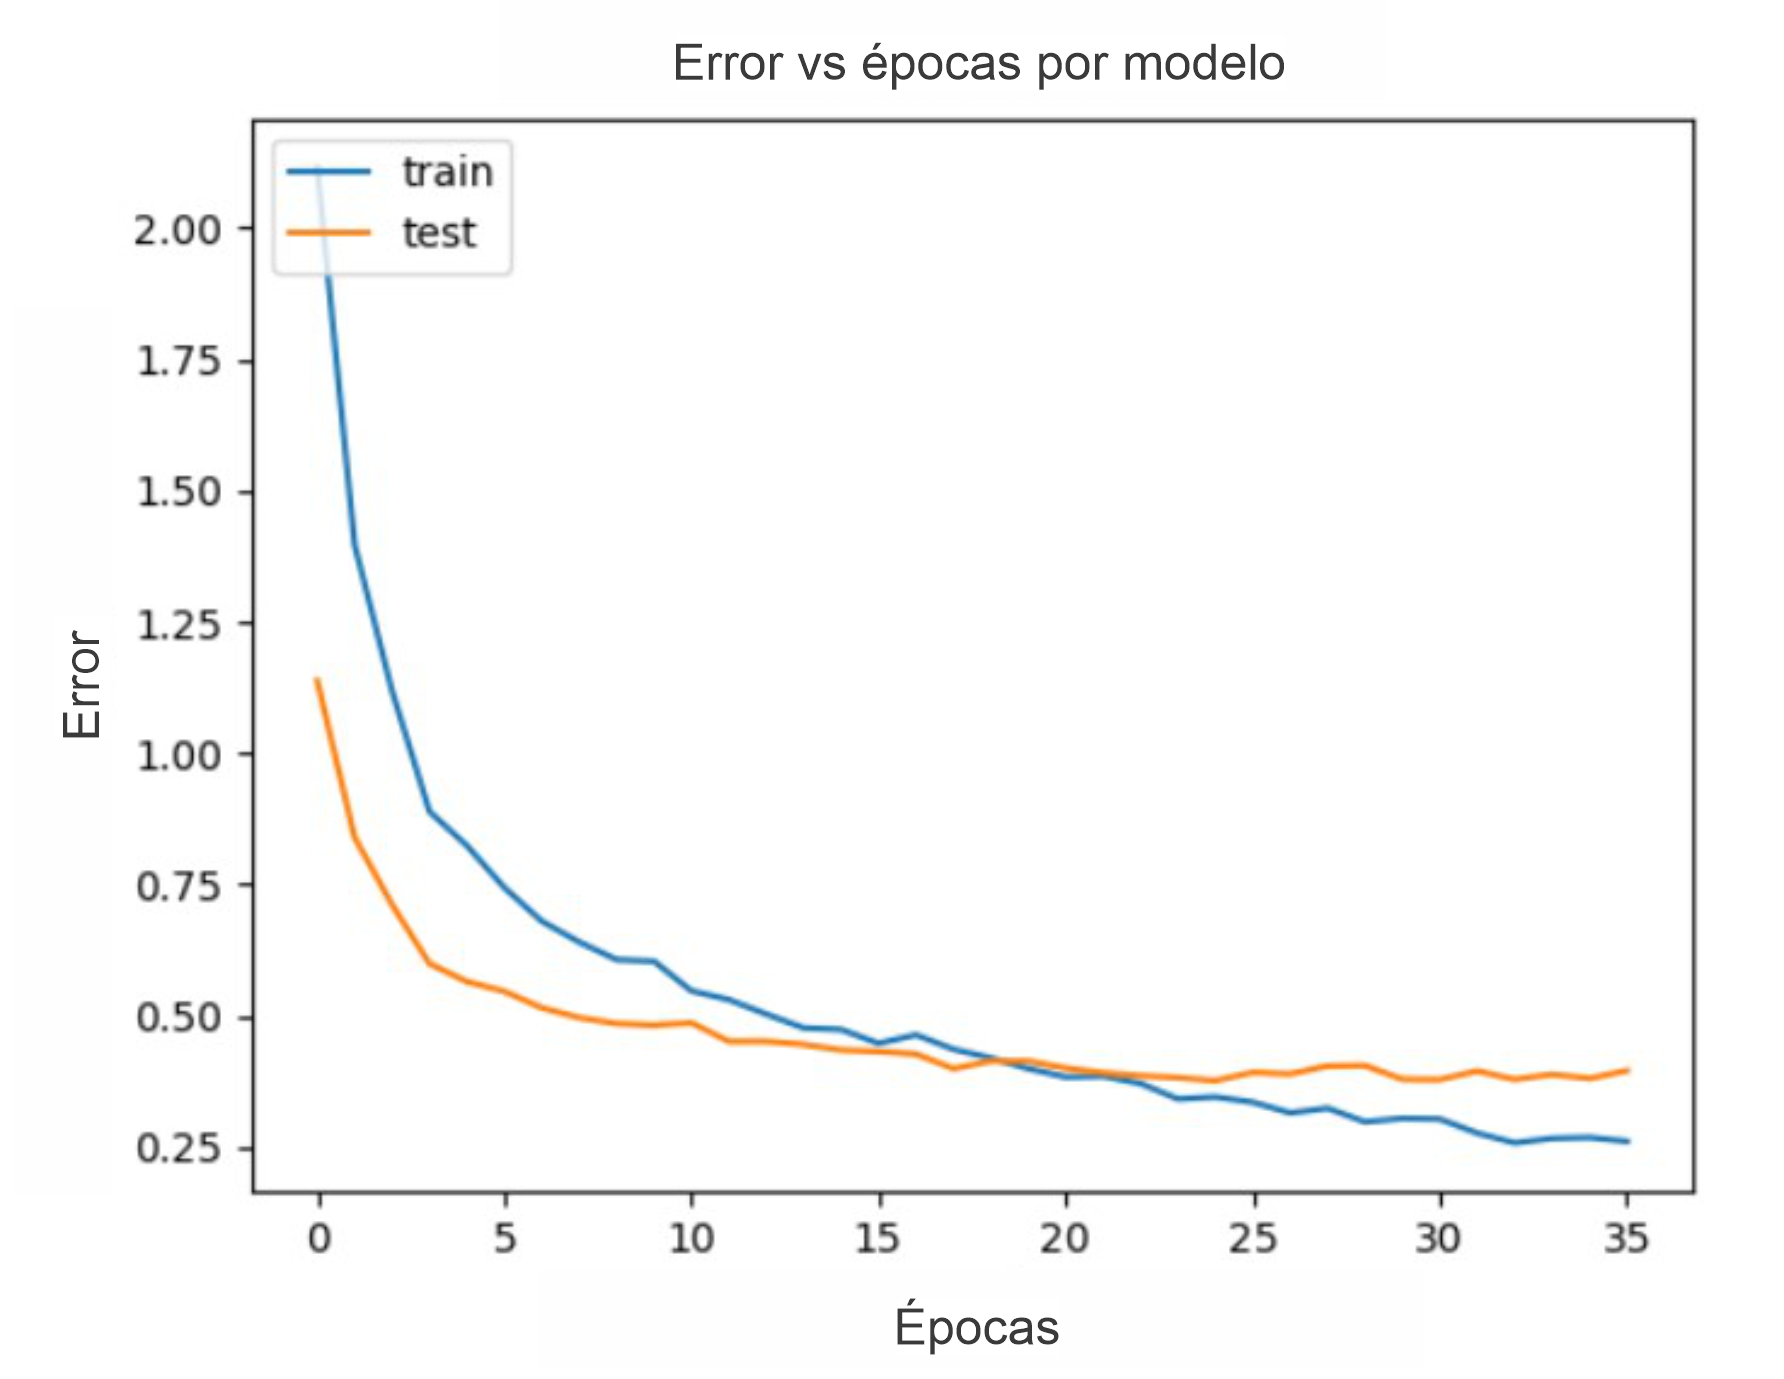
\includegraphics[width=0.8\textwidth]{images/loss5.png}
\caption{Gráfica comparativa de la perdida de entrenamiento y validacion del experimento \#3}
\label{fig:losses5}
\end{figure}

\begin{figure}[h!]
\centering
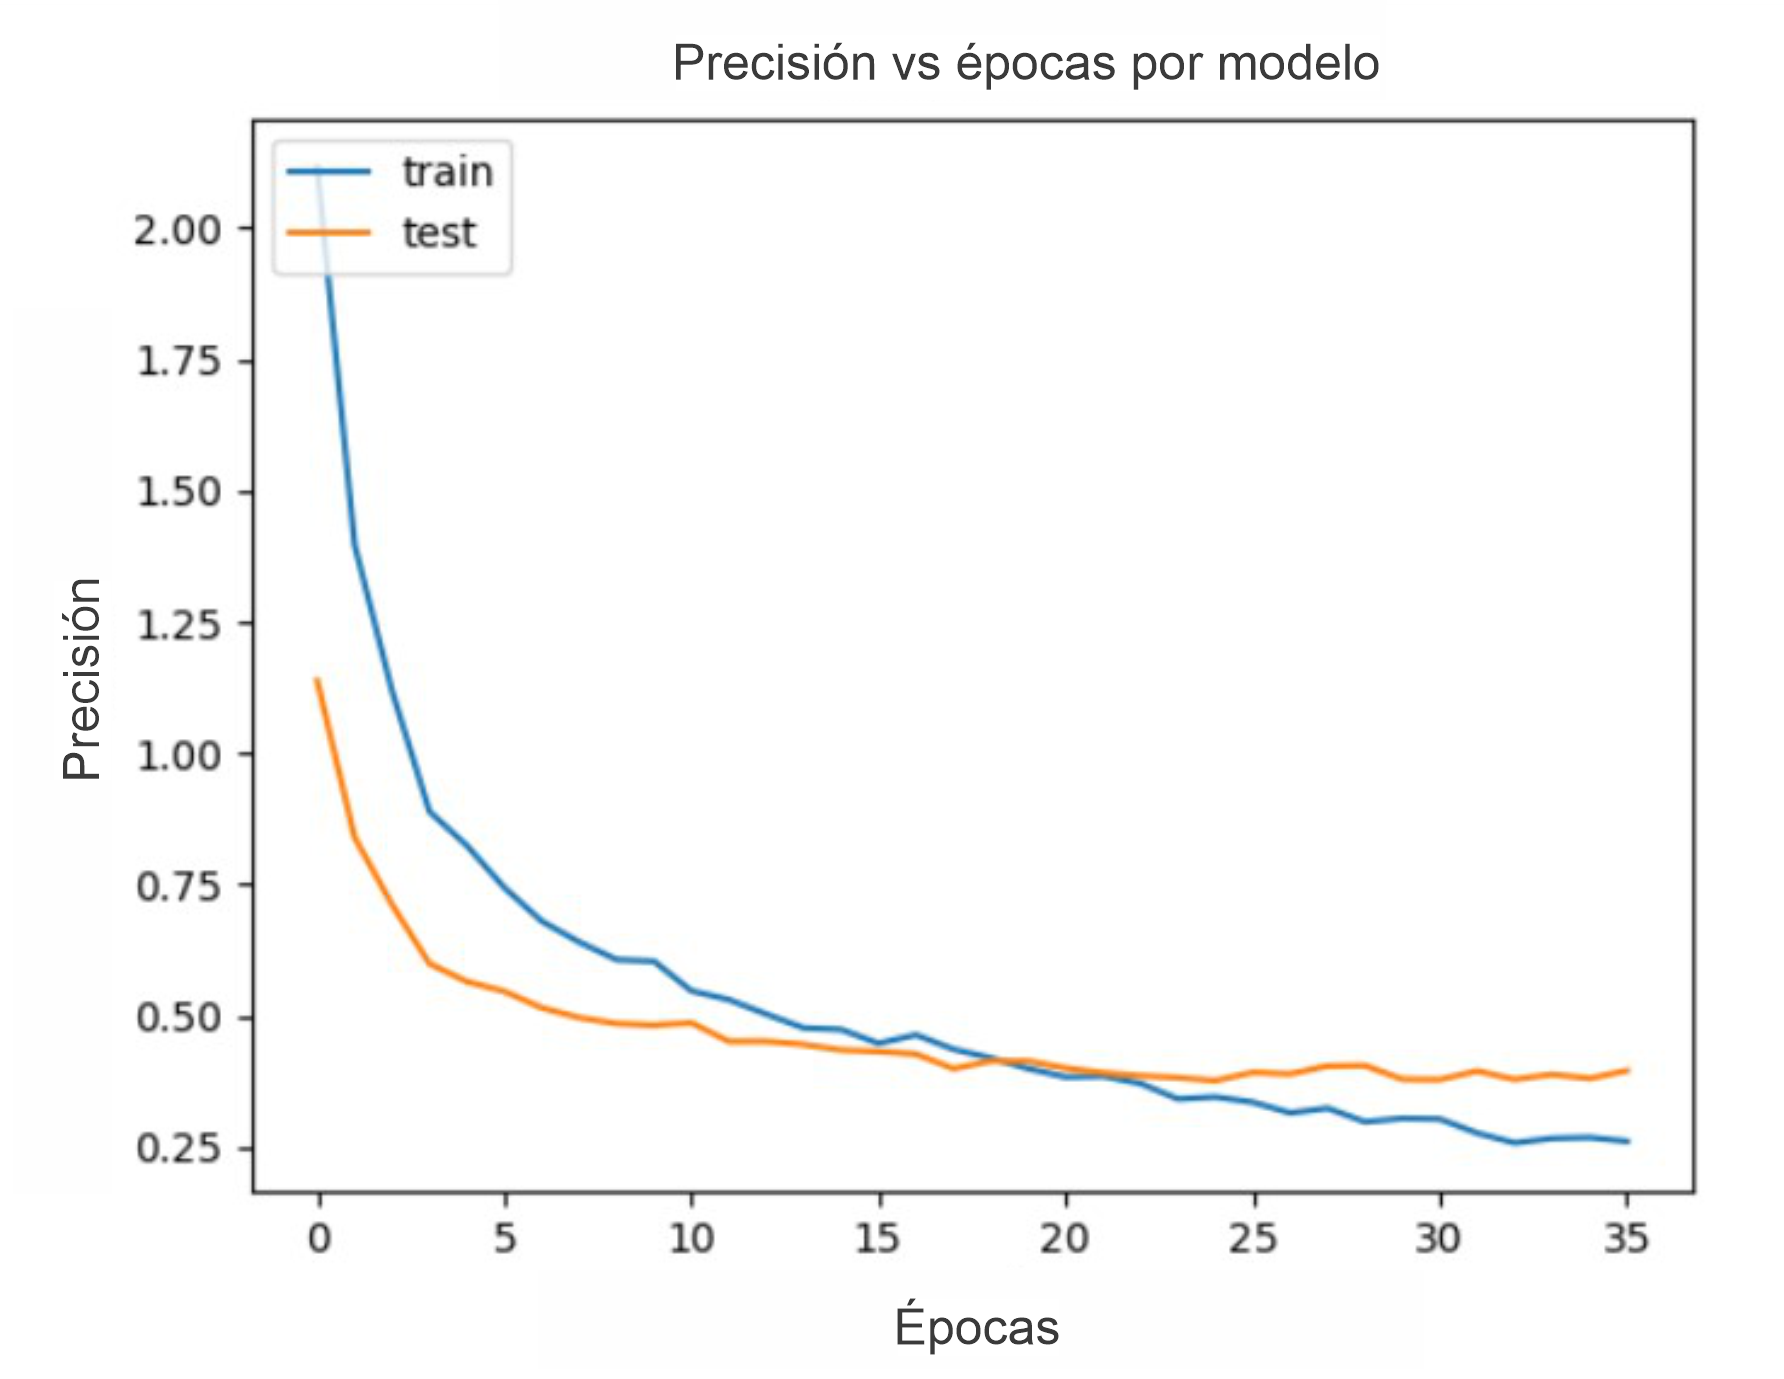
\includegraphics[width=0.8\textwidth]{images/accuracy5.png}
\caption{Gráfica comparativa de la precisión de entrenamiento y validacion del experimento \#3}
\label{fig:accuracy5}
\end{figure}

Por último, se realizó la matriz de confusión de las clases clasificadas que se pueden ver en la tabla \ref{fig:Matrix3}

\begin{figure}[h!]
\centering
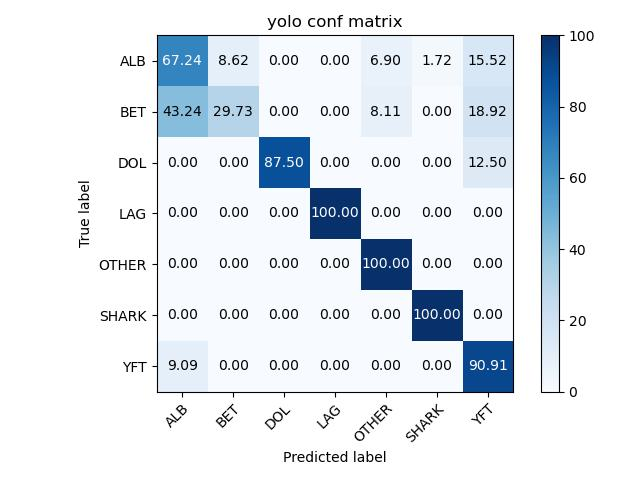
\includegraphics[width=0.8\textwidth]{images/yolo_conf_matrix.jpg}
\caption{Matriz de confusión generada por el experimento \#3 en porcentajes}
\label{fig:Matrix3}

\end{figure}

Con base en los resultados obtenidos, se puede afirmar que este modelo está preparado para ser utilizado en el \textit{pipeline} correspondiente. Es importante destacar que el entrenamiento de este modelo tardó 36 épocas, con un promedio de 10 segundos por época, lo que significa que el tiempo total de entrenamiento fue de 6 minutos, un tiempo relativamente corto. Además, el tiempo de procesamiento por \textit{batch} (32 imágenes) es de 85 ms, lo que indica que en el futuro se podría ampliar la base de datos con más imágenes de especies adicionales, para proporcionar una mayor especificidad en la detección de objetos o animales por medio del detector. En comparación, el proceso de entrenamiento para una red más compleja, que requiera una base de datos etiquetada, sería significativamente más largo y complicado.

\section{Experimentación del \textit{pipeline}}
Debido a que el \textit{pipeline} consta de dos pasos para la detección y clasificación de las imágenes, realizar una experimentación típica se hace inviable. En ese sentido, se simuló un \textit{benchmark} utilizando el flujo descrito por la imagen \ref{fig:metodologia2}

\begin{figure}[h!]
\centering
\includegraphics[width=0.9\textwidth]{images/Metodología2.png}
\caption{Flujo para la experimentación del \textit{pipeline}}
\label{fig:metodologia2}
\end{figure}

\subsection{Prueba del clasificador}

Una vez obtenidos las detecciones de los peces, quitado los errores del \textit{dataset} y etiquetar los peces que se tenían dentro del \textit{dataset} de prueba, se generaron tres nuevos \textit{datasets} de imágenes de peces detectados. Consiguientemente, se procedió a utilizar el modelo ya entrenado en la sección 5.4.3. 
A continuación se presentarán los resultados obtenidos para cada uno de los modelos, los cuales se recopilaron en la tabla \ref{table:estadisticosPipeline}.

\begin{table}[h!]
\footnotesize
\centering
\begin{tabular}{|c|c|c|c|c|}
\hline
                                                                                                                    & \textit{\begin{tabular}[c]{@{}c@{}}Balanced\\ Accuracy\end{tabular}} & \textit{F1-weighted} & \textit{\begin{tabular}[c]{@{}c@{}}Precision\\ weighted\end{tabular}} & \textit{\begin{tabular}[c]{@{}c@{}}Recall\\ weighted\end{tabular}} \\ \hline
\textit{\begin{tabular}[c]{@{}c@{}}Predicted Yolov5\\ pretrained(40\%\\ threshold)\end{tabular}}                    & 72.99\%                                                              & 68.35\%              & 76.08\%                                                               & 66.89\%                                                            \\ \hline
\textit{\begin{tabular}[c]{@{}c@{}}Predicted UniDet\\ pretrained (no \\ threshold)\end{tabular}}                    & 84.47\%                                                              & 84.67\%              & 86.50\%                                                               & 84.03\%                                                            \\ \hline
\textit{\begin{tabular}[c]{@{}c@{}}Predicted Yolov5\\ trained (freezed \\ backbone 95\% \\ threshold)\end{tabular}} & \textit{91.47\%}                                                              & \textit{91.90\%}              & \textit{91.99\%}                                                                & \textit{91.93\%}                                                            \\ \hline
\end{tabular}
\caption{Estadisticos generados por los 3 diferentes modelos}
\label{table:estadisticosPipeline}
\end{table}

Los resultados obtenidos muestran que el \textit{pipeline} funciona relativamente bien con todos los diferentes detectores, generando un \textit{balanced accuracy} bastante elevado. Por otra parte, se puede ver que los \textit{pipelines} que utilizaban los detectores preentrenados obtuvieron un resultado similar, aunque peor que el que usabe el detector entrenado. Esto es debido a que los \textit{bounding boxes} generados por el modelo entrenado coincidían con las imágenes recortadas con las que se entrenó el clasificador, mientras que UniDet generaba resultados aproximados. Por otra parte el Yolov5 preentrenado los generaba de manera muy justa, haciendo necesario que sean preprocesadas antes de ser ingresados al clasificador, por lo que también eran aproximados.
Además se obtuvieron las matrices de confusión (Tablas \ref{fig:confusionMatrix1}, \ref{fig:confusionMatrix2} y \ref{fig:confusionMatrix3}) de cada uno de los experimentos, los cuales se muestran a continuación:

\begin{figure}[h!]
\centering
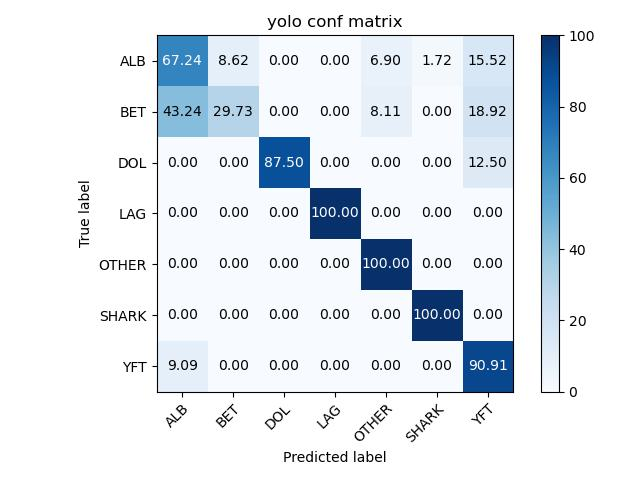
\includegraphics[width=0.8\textwidth]{images/yolo_conf_matrix.jpg}
\caption{Matriz de confusión para pruebas del \textit{pipeline} con Yolov5 preentrenado }
\label{fig:confusionMatrix1}
\end{figure}

\begin{figure}[h!]
\centering
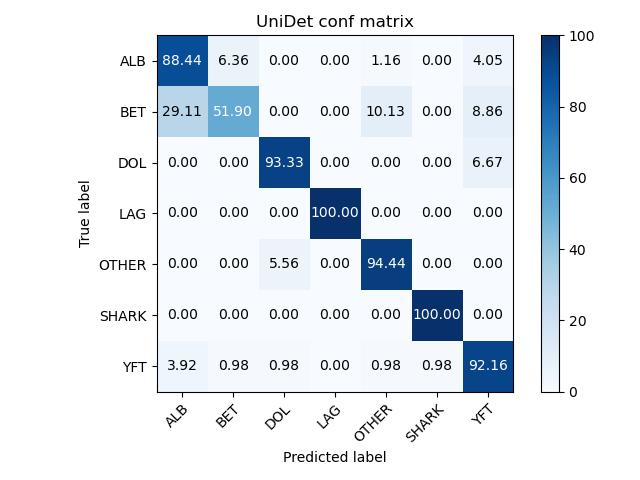
\includegraphics[width=0.8\textwidth]{images/UniDet_conf_matrix.jpg}
\caption{Matriz de confusión para el testeo del \textit{pipeline} con UnIDet preentrenado }
\label{fig:confusionMatrix2}
\end{figure}

\begin{figure}[h!]
\centering
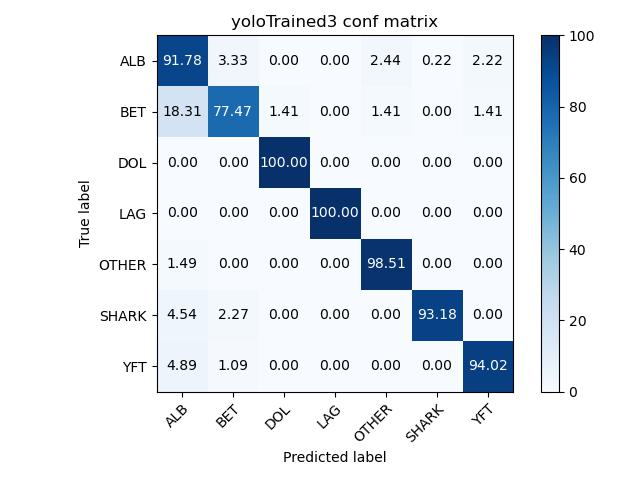
\includegraphics[width=0.8\textwidth]{images/yoloTrained3_conf_matrix.jpg}
\caption{Matriz de confusión para el testeo del \textit{pipeline} con Yolov5 entrenado }
\label{fig:confusionMatrix3}
\end{figure}
En general, se comprobó que el clasificador cumplió su función correctamente de clasificar las imágenes que le fueron proporcionadas por el detector. Aún así, la precisión de este radica en lo bien que fueron detectados los peces dentro de las imágenes. En ese sentido podemos ver que el aplicar este \textit{pipeline} generaría una pérdida en la precisión a comparación de entrenar un modelo de un 10\% a 28\% (que podría variar dependiendo del detector usado y del tratamiento de los \textit{bounding boxes}) en imágenes complejas como las que se tienen(sería conveniente realizar pruebas en imágenes menos complejas).

\section{Evaluación}

Finalmente, se comparó los resultados en términos de precisión final y el error generado de los modelos, tomando en cuenta la siguiente fórmula:
\newline
$$ precision\_final = \frac{peces\_detectados * accuracy\_clasificador}{imagenes\_reales}$$

Siguiendo esta métrica, y el porcentaje de error en la detección, se obtuvo la tabla de resultados final \ref{table:resultadosFinales}:
\begin{table}[h!]
\footnotesize
\begin{tabular}{|c|l|l|c|c|c|}
\hline
                                                                                                                    & \multicolumn{1}{c|}{\textit{\begin{tabular}[c]{@{}c@{}}Accuracy\\ parcial\end{tabular}}} & \multicolumn{1}{c|}{\textit{\begin{tabular}[c]{@{}c@{}}Accuracy \\ del \\ clasificador\end{tabular}}} & \textit{\begin{tabular}[c]{@{}c@{}}Accuracy\\ final\end{tabular}} & \textit{\begin{tabular}[c]{@{}c@{}}Porcentaje \\ de error\\ del total\end{tabular}} & \textit{\begin{tabular}[c]{@{}c@{}}Tiempo de \\ entrenamiento\end{tabular}}    \\ \hline
\textit{\begin{tabular}[c]{@{}c@{}}Predicted Yolov5\\ pretrained  (40\%\\ threshold)\end{tabular}}                  & \multicolumn{1}{c|}{14.13\%}                                                             & 72.99\%                                                                                          & 10.31\%                                                           & 69.07\%                                                                             & \begin{tabular}[c]{@{}c@{}}9 minutos\\ (CNN)\end{tabular}                      \\ \hline
\textit{\begin{tabular}[c]{@{}c@{}}Predicted UniDet\\ pretrained \\ (no threshold)\end{tabular}}                    & 40.15\%                                                                                  & 84.47\%                                                                                          & 33.91\%                                                           & \textbf{22.54\%}                                                                             & \begin{tabular}[c]{@{}c@{}}9 minutos\\ (CNN)\end{tabular}                      \\ \hline
\textit{\begin{tabular}[c]{@{}c@{}}Predicted Yolov5\\ trained  (backbone \\ freezed 95\%\\ threshold)\end{tabular}} & \textbf{79.45\%}                                                                                  & \textbf{91.47\%}                                                                                          & \textbf{72.67\%}                                                           & 32.36\%                                                                             & \begin{tabular}[c]{@{}c@{}}9 minutos(CNN) + \\ 80 minutos(yolov5)\end{tabular} \\ \hline
\end{tabular}
\caption{Accuracy final y porcentaje de errores detectados de los 3 modelos }
\label{table:resultadosFinales}
\end{table}

Considerando todos los experimentos realizados, podemos concluir que el \textit{pipeline} propuesto puede ser aplicable inclusive para casos complejos de manera que este no disminuye mucho el rendimiento de la precisión final ni aumenta mucho el tiempo de procesamiento. Además evita necesitar la obtención de un \textit{dataset} etiquetado con \textit{bounding boxes} para el entrenamiento, reducir el tiempo de entrenamiento y aumentar la escalabilidad de la especificación de especies detectadas. Cabe resaltar como punto importante que el desempeño de este \textit{pipeline} recae principalmente en poder encontrar un detector especializado o debidamente entrenado y robusto para poder detectar las diferentes clases y en el tratamiento de los \textit{bounding boxes} obtenidos para el paso por el clasificador. 